%update: Nov 21 fixed equation part. 
%update: Nov 09 by professor, rewrote all text. 
\begin{savequote}[75mm] 
It's rather easy to play any musical instrument: all you have to do is to touch the right key at the right time and the instrument will play itself.
\qauthor{Johann Sebastian Bach} 
\end{savequote}

\chapter{Nanoarchitechtonics of axial nanowire junctions of CdS and p-Si}

\newthought{A high-precision technique} was implemented to build and analyze axial nanowire heterojunctions inside a high-resolution transmission electron microscope (HRTEM). Through {\em in-tandem} using of a sharp tungsten probe as the nanomanipulator and an optical fiber as the optical waveguide the nanoscale CdS/p-Si axial nanowire junctions were constructed, and in situ recorded photocurrents from them were detected. Compared to an individual constituting nanowire, the CdS/p-Si axial nanowire junctions exhibit a photocurrent saturation effect which protects them from damage under high voltages. In addition, a set of experiments demonstrate the clear relationship between the saturation photocurrent values and the incident light intensities. The applied technique is envisaged to be valuable for bottom-up nanodevice fabrications, and the documented photocurrent saturation feature should solve the Joule heating-induced failure problem in nanowire optoelectronic devices caused by a fluctuating bias. 

\section{Introduction}
These days, key progresses in nanoscale electronics and photonics are achieved toward the significant improvement of functional device performances. Nanowires, as important building blocks in the bottom-up technology, have been shown to be prime candidates for the next generation booming nanophotonic applications because of their good crystallinity, high carrier mobility, confinement effects and infinite possibilities of assembling any required architectures for multiple purpose utilizations \cite{lieberprogramable2014,tsai2014,zhangx2014}. However, till now, fabrication of a desired nanoarchitecture employing nanoscale building blocks has been a challenge. Some nanowire-based devices, such as transistors \cite{577926446,577926447,577926448}, diodes \cite{577926449}, photodetectors \cite{577926451,tian2014photodetectors} and logic circuits \cite{577926453,577926454}, have successfully been constructed on substrates through diverse lithography techniques. By contrast, on-demand manipulation with two or more individual nanowires with a nanoscale precision and immediate creation of axial hetero-architectures made of them (for the straightforward optoelectronic tests) has never been attempted. Building of such junctions and in situ probing their optoelectronic properties would be highly valuable with respect to the “nanoarhitectonics” standpoint and uncovering novel physical properties and phenomena.\\ 

Cadmium sulfide (CdS) was reported to be one of the key materials in heterojunction type solar cell due to its advantageous type II window band structure  \cite{577926455}. Also, it was shown that the combination of CdS and Si materials results in a decent junction. Therefore many new functions and  applications may be envisioned. In addition, a careful research revealed that CdS/p-type-Si junctions are basically better than CdS/n-type-Si junctions for rectifying properties because of their specific type II band structure \cite{577926457}. Nevertheless, reliable usage of these two "hot" optical materials, i.e. CdS and Si, is rather rare, because both junction constituents are not transparent to a solar light. And the normal layered structures are considered not to be efficient. In order to directly expose the heterojunctions to the light, a smart way is to build nanowire array structures \cite{577926458,577926459}. In addition to wide-spread core-shell nanowire ensembles, constructing axial nanowire heterojunctions by means of two semiconducting materials is a promising experimental route.\\

Following previously made axial nanowire heterojunctions for diverse optoelectronic applications, CdS nanowires and boron-doped Si nanowires have been selected by me as the targeting building blocks. Thus, in this Chapter I demonstrate am accurate nanomanipulation technique pioneered  in a HRTEM for building new axial nanowire architectures. Straightforward \emph{in situ} electronic and optoelectronic tests are then carried out on them using the light of various wavelengths shining into the TEM column. The designed experiments allow me to simultaneously have an entire control over the crystallography and spatially-resolved chemistry of the two constituting domains and their interfacial region before, during and after optoelectronic probing with high spatial and temporal resolutions specifically achievable with HRTEM. 
My experiments reveal clear photosensing properties of the axial CdS/p-Si nanowire junctions. The latter demonstrate selective sensitivity to purple and blue lights rather than to the light of larger wavelengths. Also, the junctions demonstrate a photocurrent saturation effect. This implies that such junctions are applicable in detecting light intensity due to their low energy consumption and stability under unexpectedly pulsing biases. 

\section{Experimental}
\subsection{Material Synthesis}

\begin{figure}  
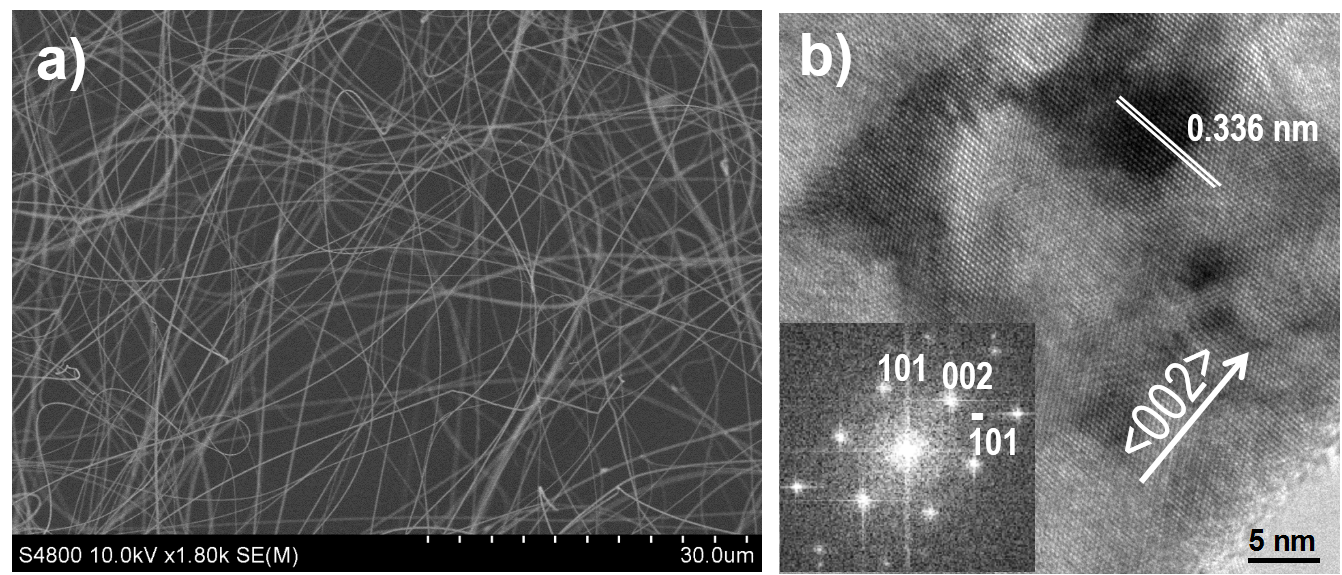
\includegraphics[width=\textwidth]{figures/figure3_s1}
\caption[SEM and TEM of CdS nanowires.]{SEM and TEM of CdS nanowires.
\label{fig:fig3_s1}}
\end{figure}

The CdS nanowires were prepared using an Au-catalyzed vapor-liquid-solid (VLS) growth  in a chemical vapor deposition (CVD) system, which is similar to that used in the previous works \cite{zhang2014photosensing,577926461}. One gram of CdS powder (99.995 percent) was placed on a graphite plate at the center of a tube furnace as the source material. A (100) silicon wafer covered with a 10 nm thick Au layer was put on the other graphite plate located downstream, at a distance of 11.5 cm from the tube center. The tube was purged under nitrogen flow at 200 °C for 2 h, and then heated to 1000 °C at a rate of 30 °C per min. After 30 min of reaction, the furnace was naturally cooled down to room temperature. The process took place under a \ce{N2} flow of 300 sccm. A wool-like yellow product was found on the Si substrate after cooling. 
Si nanowires were fabricated via VLS mechanism in another CVD system. Gold particles of 3 nm in diameter were taken as a metal catalyst. The B-doped nanowires were directly grown onto Au-coated (111) Si substrates at 600°C for 30 min in a flowing 19 sccm of \ce{SiH4} as a Si reactant gas and diborane \ce{B2H6} was employed as a B precursor. The \ce{B2H6} flow in \ce{H2} was 0.2 sccm and 30 sccm of nitrogen \ce{N2} served as the carrier gas. More details on B-doped Si nanowires characterizations were described in the literature. \cite{577926462,577926464,577926465}.

\begin{figure}  
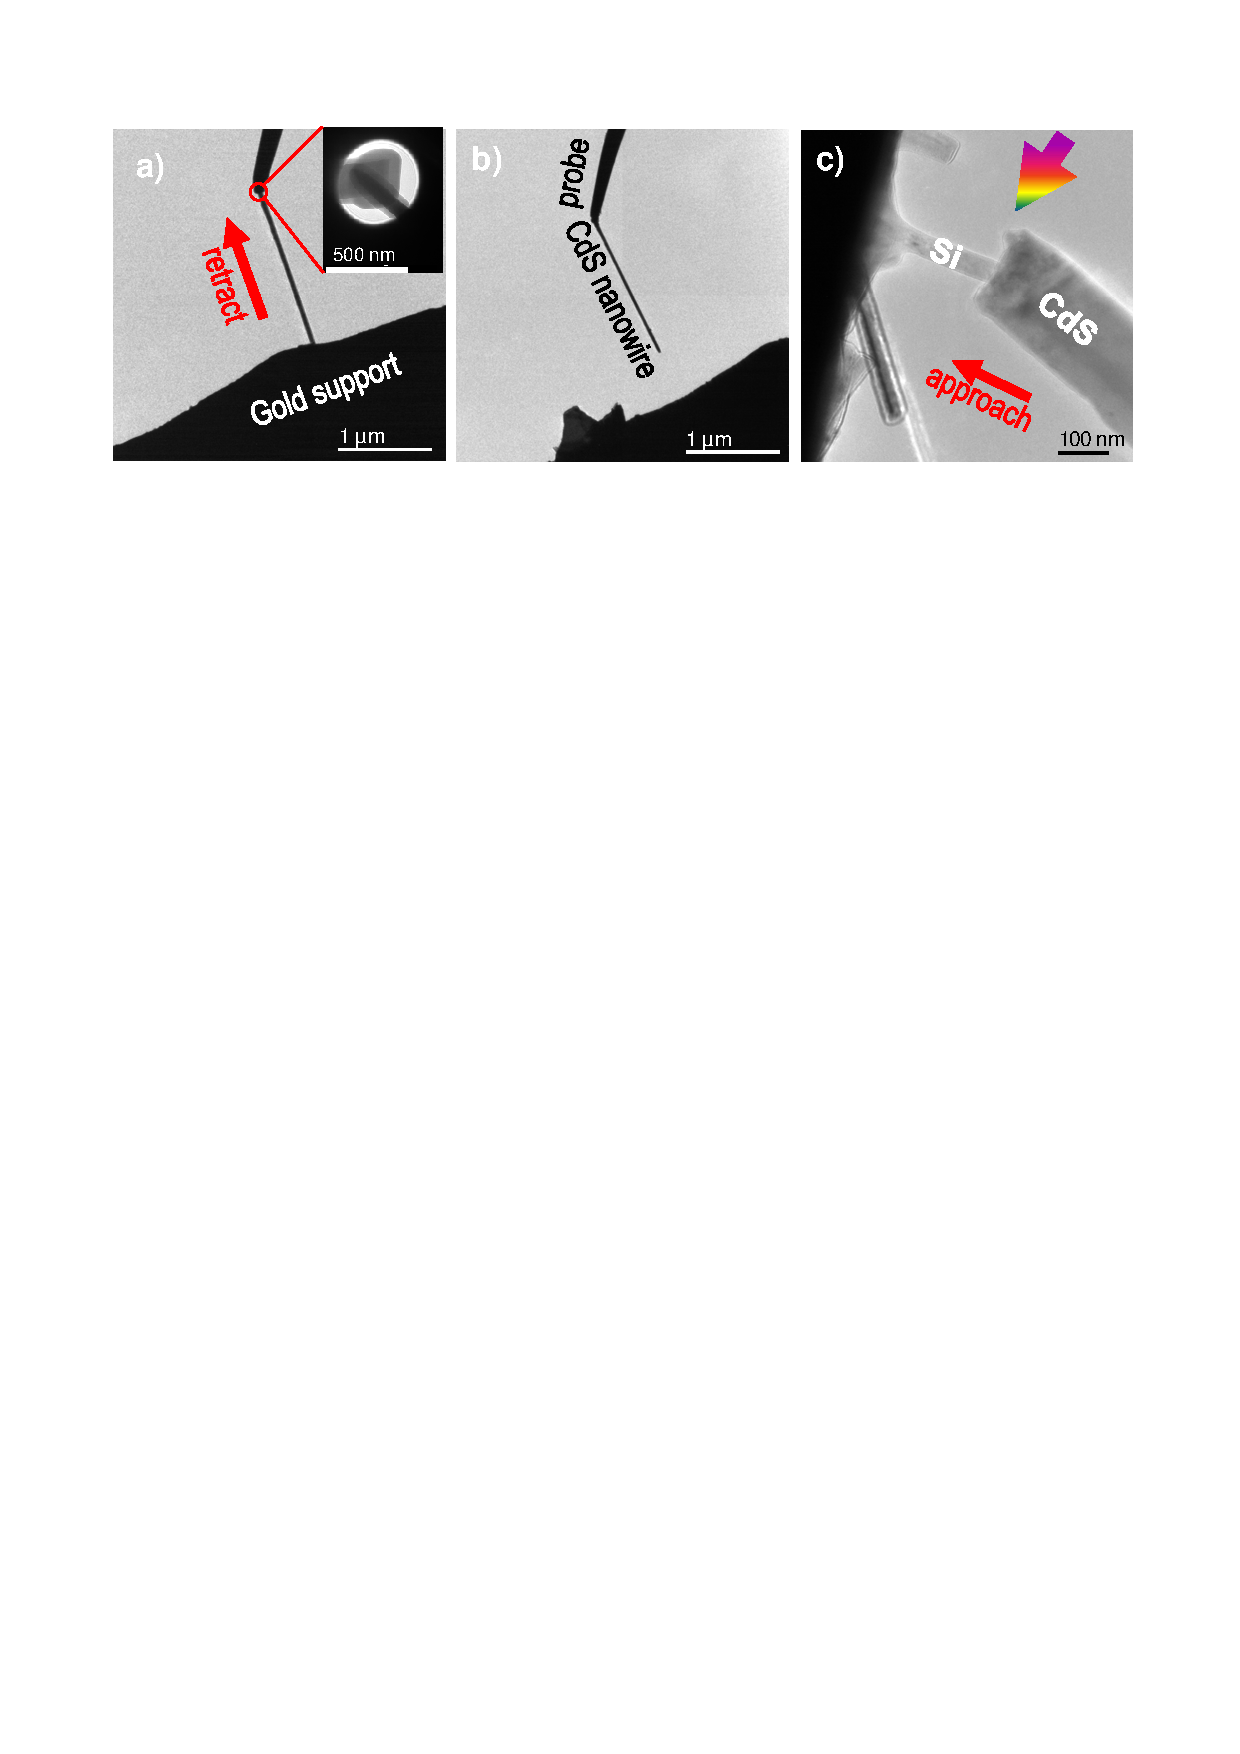
\includegraphics[width=\textwidth]{figures/figure3_1}
\caption[To make an axial junction.]{To make an axial junction.
\label{fig:fig3_1}}
\end{figure}

\subsection{Techniques}
Field-emission scanning electron microscopy (FE-SEM) of the fabricated nanostructures was performed on a Hitachi S-4800 FE-SEM operated at 10 kV. HRTEM analysis and in situ experiments were conducted using a modified piezo-driven optical TEM holder (Nanofactory Instruments AB) in an energy-filtering 300 kV JEM 3100FEF (Omega Filter) high-resolution TEM, figure \ref{fig:fig3_1}. The multimode fiber (Nanonics Imaging, Ltd.) was threaded through the holder inner channel. The fiber was connected to four laser diodes, with 405, 488, 638 and 808 nm wavelengths, and a tunable power and temperature (Thorlabs, Inc.) were used, as shown in figure \ref{fig:fig3_1}. The working temperatures of laser diodes were fixed at 30°C. First, the numerous CdS nanowires were placed onto a fresh-cut flattened Au tip covered with an electrically conductive Ag epoxy under the flash tip immersing into the CdS nanopowder sample. After heating the paint, the Au tip with the specimen was placed within the sample holder. The sharp W probes used as counter-electrodes and nanomanipulators were prepared under NaOH electrochemical etching. The W tip movements were controlled inside TEM in 3 dimensions using a piezoelectric motor for making a contact, and to test and retract the selected CdS nanowires which had been conveniently oriented with respect to the manipulator. Then the fabrication of axial CdS/p-Si nanowire junctions was gently performed in two steps, as described in the following section. Typically, before contacting the two nanowire building blocks, an electron beam was applied to focus on the tip-ends of both CdS and p-Si nanowires for 30 s to clean the surfaces at a high current density. The current–voltage (I–V) measurements were carried out by a Keithley 2612B sourcemeter. The electron been was always turned off during the electrical and optoelectronic tests. 

\begin{figure}  
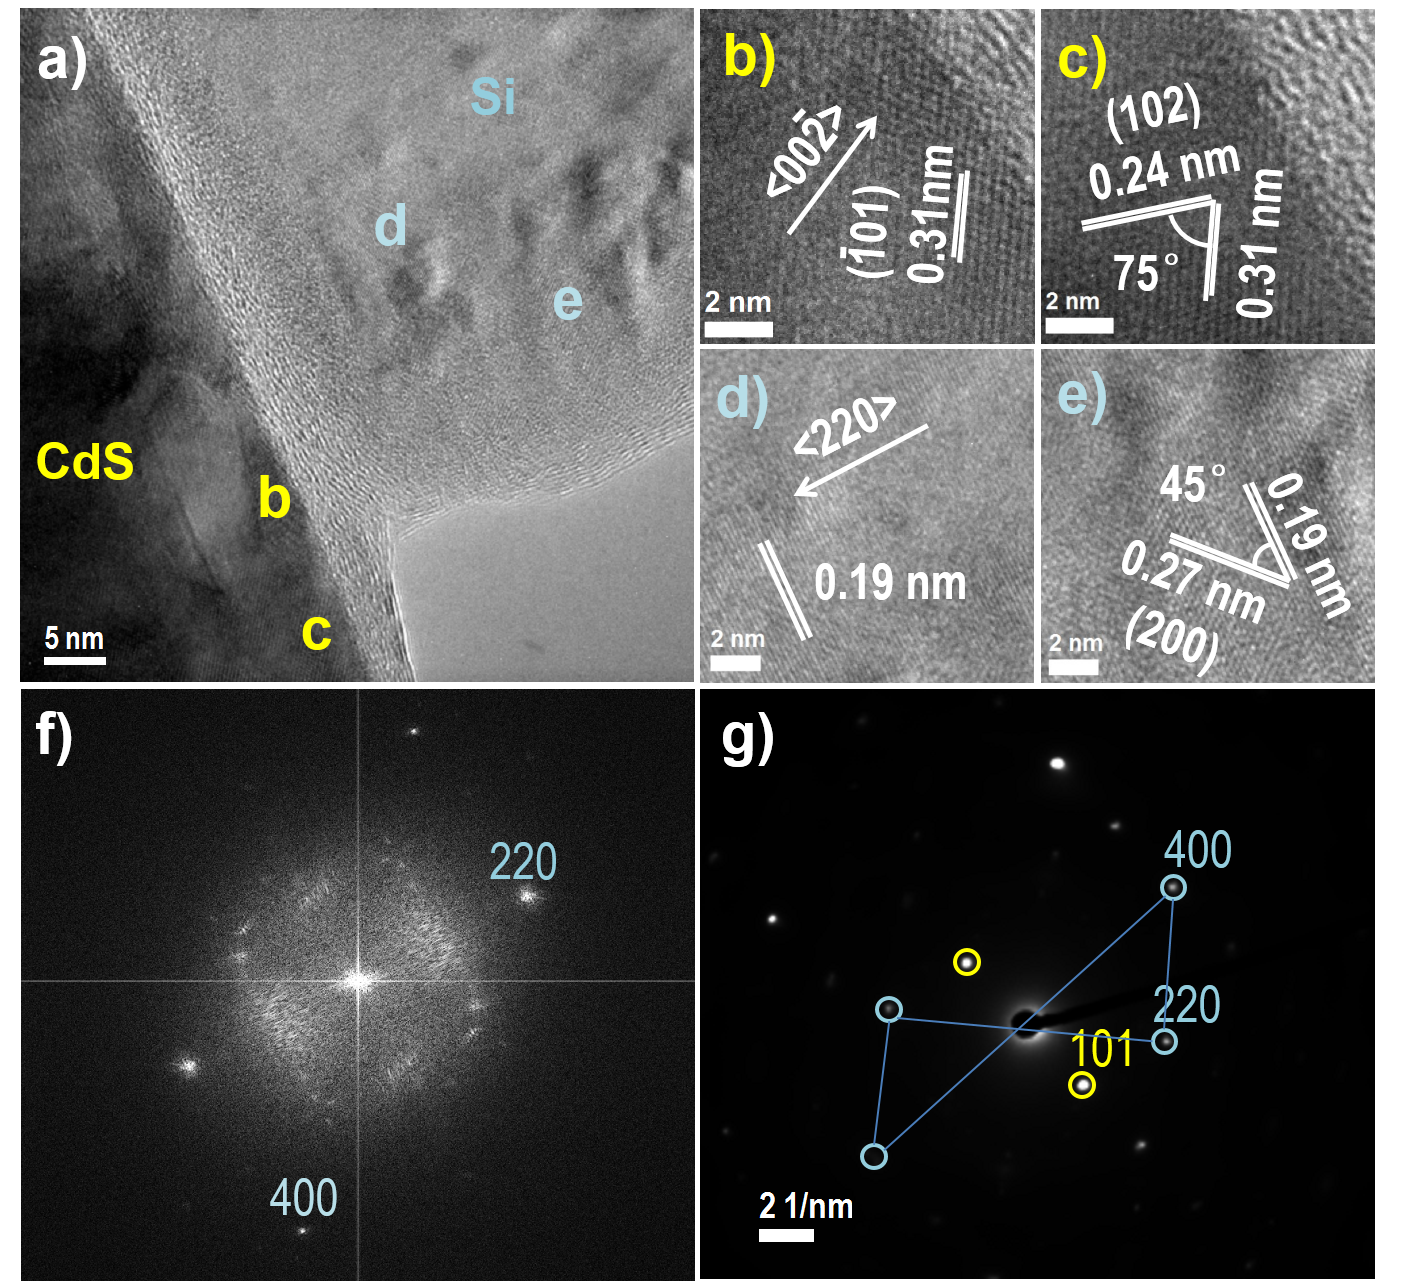
\includegraphics[width=\textwidth]{figures/figure3_2}
\caption[HRTEM anaysis on junction.]{HRTEM anaysis on junction.
\label{fig:fig3_2}}
\end{figure}


\section{Results and discussions}
As shown in the SEM image of figure \ref{fig:fig3_s1}a, fabricated CdS nanowires, more than 50 μm long, are evenly distributed over a Si substrate within a large area. In figure \ref{fig:fig3_s1}b, a high-resolution TEM image and the fast Fourier transform pattern (FFT) confirm that an individual nanowire has a well-crystallized hexagonal structure. The growth direction is along the c-axis and the lattice constant c = 0.672 nm. 
Since the deoxidized Si nanowires are less stable than CdS nanowires in air, for constructing heterojunctions, it was important to transfer a CdS nanowire into the HRTEM first, and then to contact a Si nanowire, not vice versa. As shown in figure \ref{fig:fig3_2}a, the sharp W probe was precisely manipulated inside HRTEM to contact a pre-selected clean individual CdS nanowire on the Au stage. To pull out the CdS nanowire from the sample stage, an electron-beam soldering, i.e. "glue" technique, was utilized for making the tight contact between the probe and the nanowire. As illustrated in the inset of figure \ref{fig:fig3_2}a, by focusing a convergent electron probe (about 0.5 microns in diameter) on the contact area for 20 min, nearly 75 nm thick layer of the residual amorphous carbon (always present in the TEM chamber from lenses, apertures etc.) formed on the probe/nanowire surfaces  resulting in their intimate nano-soldering. Then, the targeted CdS nanowire was detached from the Au sample tip under delicate pulling back the W probe, as shown in figure \ref{fig:fig3_2}b. To bulid a final heterojunction, the second step was to contact the pulled-out CdS nanowire with an individual pre-selected boron-doped-Si nanowire. To do so, after retracting the sample holder (with the regarded CdS nanowire on the tungsten probe) from the microscope, the gold sample stage with CdS nanowires was replaced in HRTEM by the fresh Au sample stage with attached numerous deoxidized B-doped Si nanowires. By precisely approaching and contacting the end of the CdS nanowire probe to a selected Si nanowire tip, the axial heterojunction architectures were formed. Figure \ref{fig:fig3_2}c depicts a typical CdS/p-Si axial nanowire junction. These representative CdS and Si nanowires have diameters of ~187 nm and ~46 nm, respectively. The electron beam intensity was immediately weakened after the junction had been constructed. This was done to avoid the nanostructure overexposure to the electron beam which would lead to insurmountable structural changes, e.g. appearance of irradiation-induced defects in the nanostructure.

\begin{figure}  
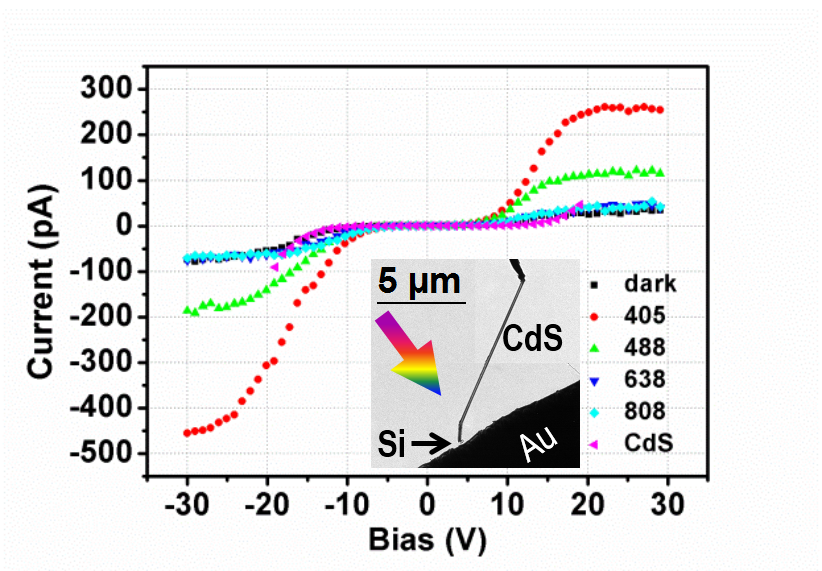
\includegraphics[width=\textwidth]{figures/figure3_3}
\caption[Photocurrent through junction.]{Photocurrent through junction.
\label{fig:fig3_3}}
\end{figure}

Then a detailed structural study of the junction was conducted using imaging and electron diffraction analysis. The HRTEM images of a representative CdS/p-Si axial heterojunction are depicted in figure \ref{fig:fig3_3}. These confirm that both nanowires are perfectly-structured single-crystals. The contact of two nanowires is atomically smooth. Unintentional thin merging graphitic layer is noticed between the wires. It has the origin similar to that mentioned above. In figure 3a, the left-hand-side panel shows the CdS nanowire, while the right-hand-side reveals the boron-doped Si nanowire. Figures \ref{fig:fig3_3}b and \ref{fig:fig3_3}c depict the full crystallographic details of the CdS branch. Figure \ref{fig:fig3_3}d and \ref{fig:fig3_3}e present the crystal lattice of the constituting Si nanowire. Figure \ref{fig:fig3_3}f is the fast Fourier transform pattern of figure \ref{fig:fig3_3}a. Figure \ref{fig:fig3_3}g is the selected area diffraction pattern taken at the junction interfacial region. After the complete structural characterization, which confirmed that high-quality axial heterojunction, made of two single-crystalline defect-free pure nanowires, had indeed been prepared, electronic and optoelectronic tests on it were promptly started. 
By applying a bias and illuminating the preformed CdS/p-Si heterojunction with a light through the optical fiber inserted into the holder, dark current and photocurrent measurements were accomplished. Figure 4 illustrates a typical current – voltage diagram of a junction illuminated with lasers of four different wavelengths. The powers of all laser diodes were fixed to be the same, 13 mW. A photocurrent of the junction at 405 nm was higher than that of 488 nm, and much higher than those at 638 nm, and 808 nm, and the dark current. Since laser diode wavelengths of 405 nm, 488 nm, 638 nm and 808 nm correspond to energies of 3.06 eV, 2.54 eV, 1.94 eV and 1.53 eV, respectively, while CdS and Si nanowire band gaps are ~2.4 eV and ~1.5 eV, respectively, \cite{Fabbri2014}, the heterostructure light absorption at 3.06 eV and 2.54 eV should be easier than that at the energy below 2.4 eV. The higher photoresponse at 3.06 eV than that at 2.54 eV could reflect a complex band diagram of the heterostructure which gives more light absorption possibilities at the higher energy, and hence results in more photo-induced carriers. 



\begin{figure}  
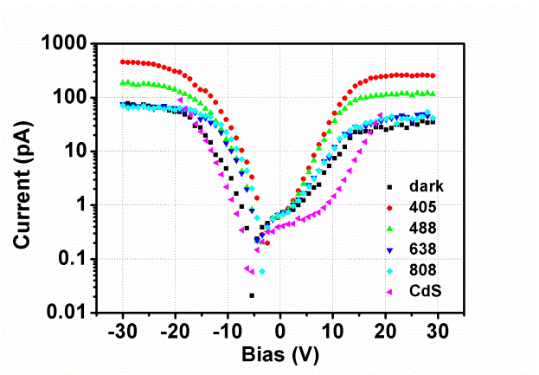
\includegraphics[width=\textwidth]{figures/figure3_4}
\caption[Photocurrent in Log scale.]{Photocurrent through junction in Log scale.
\label{fig:fig3_4}}
\end{figure}

\begin{figure}  
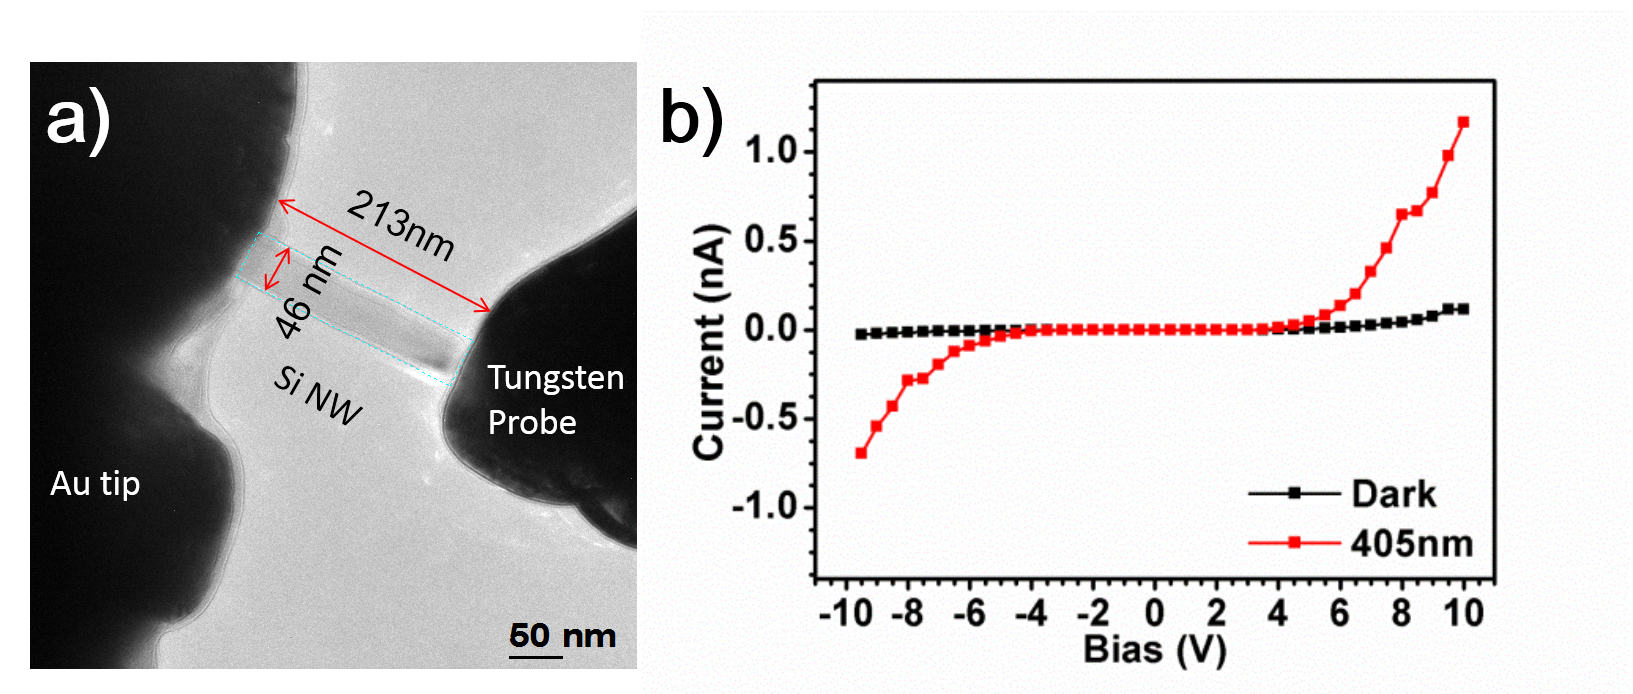
\includegraphics[width=\textwidth]{figures/figure3_s2}
\caption[HRTEM anaysis on junction.]{HRTEM anaysis on junction.
\label{fig:fig3_s2}}
\end{figure}


The current-voltage curves of the CdS/p-Si axial junction, where CdS is considered to be an n-type semiconductor (due to S vacancies), and B-doped Si as a p-type semiconductor, did not show an ideal p-n junction parameters. In the forward bias regime, below 10 V, the I-V curves reveal small currents, and the currents become saturated at a bias higher than 20 V. In the reverse bias regime, the currents also exhibit a saturation tendency, over 30 V. To compare, for a single CdS nanowire or a B-doped Si nanowire, saturation did not occur up to 10 V, as shown in figure \ref{fig:fig3_4} and figure \ref{fig:fig3_s2}. When a bias larger than 10 V had been applied to a single CdS or Si nanowire, their structural breakdown readily occurred. This was due to Joule heating at a high current density. \cite{Wu2004} In my experiments, the single crystalline nanowires (having small contact areas with electrodes) were particularly vulnerable to current densities higher than ~104 $A\cdot cm^{-2}$. Therefore, it is apparent that the CdS/p-Si junction effectively restricted the current density at a high bias, and thus protected structures from damage. 

\begin{figure}  
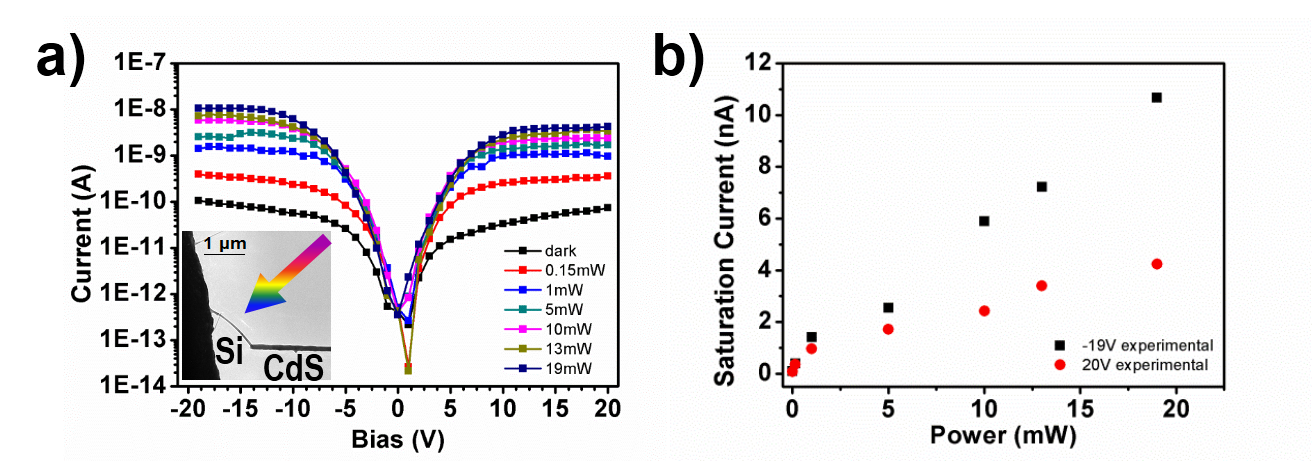
\includegraphics[width=\textwidth]{figures/figure3_5}
\caption[Photocurrent at different power.]{Photocurrent at different power.
\label{fig:fig3_5}}
\end{figure}

\begin{figure}  
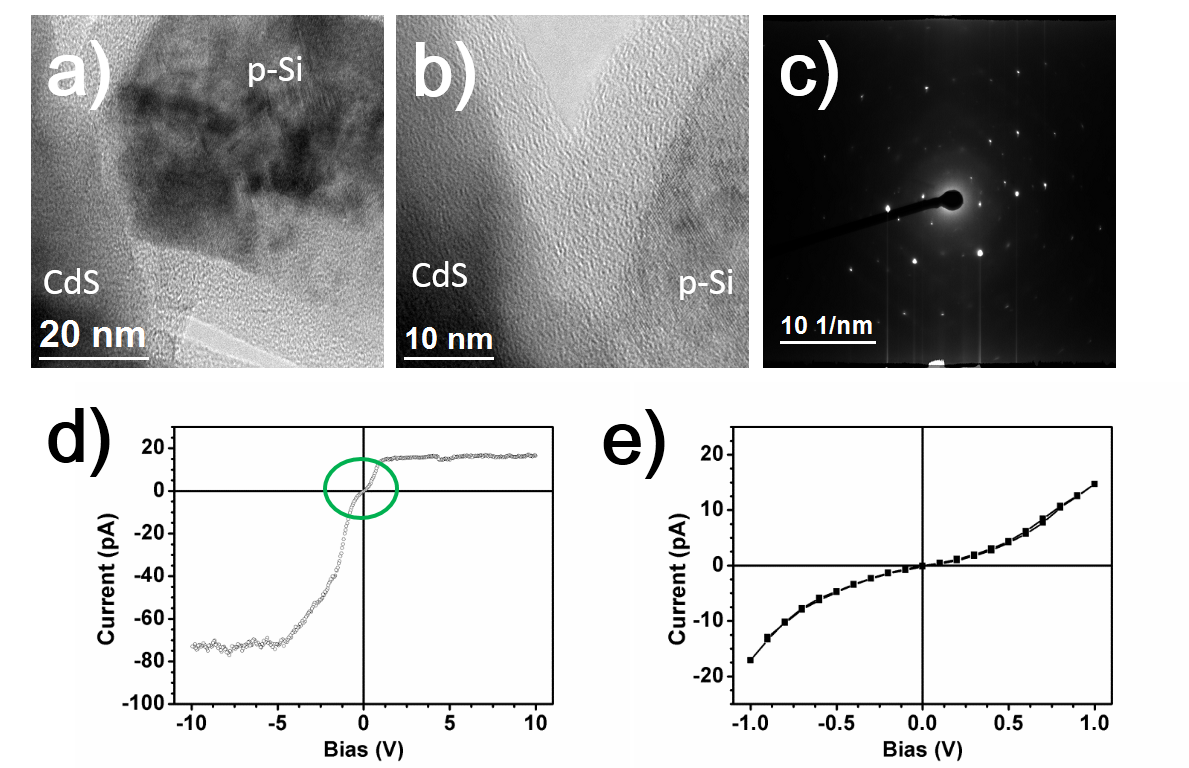
\includegraphics[width=\textwidth]{figures/figure3_s3}
\caption[HRTEM analysis on junction.]{HRTEM analysis on junction.
\label{fig:fig3_s3}}
\end{figure}

Test experiments were performed to understand the relevant factors responsible for current saturation. As shown in figure \ref{fig:fig3_5}, by measuring  photocurrents at different light intensities at 488 nm, we found that photocurrents and dark current of the CdS/p-Si axial nanowire junction at different laser power levels were accordingly saturated. The saturated currents stayed in proportion to the laser diode power. Such phenomenon implies that the CdS/p-Si junction transfers light intensity into an electrical signal with the excellent voltage tolerance. As shown in figure \ref{fig:fig3_s3}, another junction with a smaller contact area, which was illuminated by a 405 nm laser at 13 mW, also demonstrated a profound saturation effect. The photocurrent saturated at 5 V, the saturation current values were 15 nA and –75 nA. Therefore, it is likely that the junction contact conditions largely affect the saturation threshold and the current value. Generally, the photocurrents of nanowire photodetectors are proportional to the voltage \cite{577926470}[29], while, at the same time, they are proportional to the light intensity. This means that the voltage should certain and stable within a limited tolerance for reliable light detection. Consequently, the presently built CdS/p-Si axial nanowire junctions show a great promise toward light intensity sensing not only because they can restrict the current density at a high voltage, but also because they do not need an entirely stable voltage. 
The observed phenomenon of photocurrent saturation at high bias levels appears to be analogous to that reported for a planar Metal-Semiconductor-Metal (MSM) photodetector \cite{577926472}, electron beam excited CdS single crystals \cite{577926473}, a model p-n junction photocurrent \cite{577926474} and a p-n junction solar cell \cite{Gu2005}. First, the electron beam excitation mechanism should be excluded, because the electron beam was turned off during the measurements, and the electron beam does not have a continuous effect on a photocurrent of the material \cite{577926473}. Second, the as-synthesized CdS nanowires had been verified to be a defect-free crystals with a limited number of S vacancies, and, hence, they did not operate as a heavily doped donor. For an ideal p-n junction, the dark current could be expressed as: 
$$I=I_s\left(e^\frac{V_D}{nV_t}-1\right)\eqno{(1)}$$

Equation ($1$) is called Shockley’s diode equation \cite{577926477} and the dark current density of a non-ideal diode could be written as: 
$$J_F\approx-\frac{q(2D_p)N_i}{L_p}e^\frac{qV}{mk_0T}\eqno{(2)}$$
The factor m in Equation ($2$) is changeable. Under circumstances of very low and very large biases, $m = 2$, and $J_F\propto e^\frac{qV}{k0T}$, the recombination current or the high injection takes an effect, current densities increase linearly; when bias is on a medium level, $m=1$, $J_F\propto e^\frac{qv}{2k0T}$, the diffusion current becomes important, and the current density exponentially increases. This is similar to the observed I-V curve trends, but Equation (2) does neither exactly explain the photocurrent saturation phenomenon nor the relationship between the saturation current value and incident light intensity. From the theory of photocurrent saturation proposed by Mohammad and Abidi \cite{577926474}, for lightly degenerated semiconductors, where spatial variations of dielectric constant, effective mass, carrier lifetime, mobility and diffusivity are significantly small and could be neglected, the total current could be expressed by: 
$$I=Aqg\left ( L_{n}^{*}+L_{p}^{*} \right )-\frac{\left ( e^{\frac{qV_j}{kT}-1} \right )\cdot \left (  I_0+I_{0}^{'} e^{-z} \right )}{1-e^{-2z+z_1+z2}}\eqno{(3)}$$
where, 
$$I_0=\frac{qA}{\tau_a}(n_0(x_{p2})L_n^*+p_0(x_{n2})L_p^*)$$
$$I_0=\frac{qA}{\tau_a}(n_0(x_{p2})L_p^*e^{z2}+p_0(x_{n2})L_n^*e^{z1})$$
$$L_n^*=L_p^*=L_a=\sqrt{D_a\tau_a}$$
$D_a$, $\tau _{a}$ and $g$ are defined as ambipolar-diffusion coefficient, ambipolar lifetime and amibipolar-carrier generation rate in ref [33], respectively. We do not neglect injection, $V_j, V_d$, and  it is considered that $z_1=z_2=0$, $z=\frac{q}{kT}(V_d-V_j)$ in nondegenerated semiconductors with uniform doping, Equation (3) could be written as: 
$$I=2qAg\sqrt{D_a\tau_a}-k_v(n_0x_{p2}+p_0x_{n2})$$
$k_v$ is defined as factor to simplify the equation. The first term on the right-hand side of this Equation represents the uncompensated current relative to light intensity, and the second term expresses the reduction of this photocurrent owing to spatial dependence of band structure of the junction and the junction potential produced by high injection. For a single B-doped Si or a defect-free CdS nanowire, the current densities increase with bias, as these do for a normal semiconductor nanowire with Schottky contacts. However, for the CdS/p-Si nanowire junctions with a small junction area and under large bias, the second term of Equation (4) becomes insignificant, and therefore the photocurrent does not rise with a bias but does with the light intensity. 
The observed saturation current values in correspondence with incident light intensities could be ascribed to the several reasons. Since a sufficient bias must be applied to have the flat band at the anode and separate the generated carriers, after the threshold bias, the photocurrent started to notably raise, but when the bias is large enough, effective carriers generated by the incident light become saturated for transmission. Also, we propose that the CdS/p-Si axial nanowire heterostructures are quite sensitive to 3 factors: the relative sizes of the two building blocks (that affects carrier mobility), carrier density and light absorption efficiency; interface crystallography, which also affects mobility, junction parameters; and light intensity; which affect the saturation photocurrent value. 
Over this work I fabricated and thoroughly tested 5 different CdS/p-Si nanowire junctions. All of them exhibited the above-discussed saturation effects with somewhat varying parameters, as documented in Table 1. The results confirmed that the saturation effect is natural and highly reproducible in an \emph{in situ} TEM. 

\section{Conclusions}
To sum up, a direct in situ HRTEM technique to construct individual axial nanowire junctions (perfectly highlighting the popular “nanoarchitectonics” concept) has been for the first time demonstrated. In situ HRTEM and in-tandem structural characterizations and optoelectronic tests highlight the photosensing properties of the single-crystalline axial CdS/p-Si nanowire junctions. The junctions exhibit good selectivity toward the light frequencies higher than those of the yellow range. The junctions possess a specific photocurrent saturation effect; this could be utilized in low-consumption light intensity sensing and integrated tunable voltage-driven applications thanks to the corresponding current limitations and excellent tolerance toward possibly unreliable and unstable bias. Clearly, the present nanoarchitectonics-based approach employing in situ structural design and measurements gives a strong motivation for establishing new operational principles of single crystal nano-devices. Furthermore, it is also envisaged that the near-field scanning technique could be also integrated within the designed system for even deeper understanding of the exciting nanoscale optoelectronic phenomena.\cite{Gu2005,Xiang2012}.



